
\section{Experimentos}

\begin{frame}
\frametitle{Setup de training}
Recapitulando... ¿Qué hay que definir para entrenar una red? \pause
\begin{itemize}
\item \textbf{Feature set}: determina la codificación y los patrones que se pueden aprender \pause
\item \textbf{Dataset}: datos de entrenamiento, visto anteriormente \pause
\item \textbf{Arquitectura de la red}: el tamaño de cada capa; $L_1$ y $L_2$ \pause
\item \textbf{Método de entrenamiento}: PQR/target scores; determina el formato de las muestras y la loss function  \pause
\item \textbf{Hiperparámetros}: learning rate, batch size, epochs, etc.
\end{itemize}
\end{frame}

\begin{frame}
\frametitle{Setup de evaluación}
¿Cómo evalúo el performance de una red entrenada? \pause
\begin{itemize}
\item \textbf{Loss} (train y val.): indica la calidad de las predicciones.
\begin{itemize}
    \item Permite detectar overfitting y otros problemas \pause
\end{itemize}
\item \textbf{Puzzle accuracy}: porcentaje de movimientos acertados en puzzles de Lichess.
\begin{itemize}
    \item Sólo hay un movimiento correcto
    \item Proxy (muy malo) de la fuerza de la red \pause
\end{itemize}
\item \textbf{Elo relativo}: la medida más común para comparar engines.
\begin{itemize}
    \item Se realizan torneos de 100ms por movimiento
    \item El elo es calculado a partir de Ordo
\end{itemize}
\end{itemize}
\end{frame}

\subsection{Baseline}

\textbf{Motivation.} Experiments that will follow will focus on trying out different feature sets, so it is natural to keep every other variable constant. Since the dataset is fixed and the feature set is going to be changing, it remains to find acceptable values for the network architecture and the training hyperparameters. 

Due time and resources constraints, I decided to set the training hyperparameters to   (similar) values which give good results in the official Stockfish trainer: \textbf{a batch size of 16384, a learning rate of 0.0005 and a exponential decay factor of 0.99}. This values showed acceptable results during early stages of development and will remain fixed for all runs.

It remains to find a good network architecture. Bigger networks may have lower loss and predict better, but they will also have slower inferences. This is the tradeoff between inference time and node visits (more depth), which are also affected by the quality of the prediction due to better pruning. So the model must be so much better to compensate the slowdown in inference. \\

\textbf{Experiment.}  In this first experiment I will try different sizes of L1 and L2,  to find an acceptable tradeoff for future experiments. I will run a grid search with L1 $\in \{256, 512, 1024, 2048\}$ and L2 $\in \{32, 64, 128, 256\}$. The feature set used to train will be \featureset{All}, the canonical set with 768 features.

I expect that there will be a model that performs best and other models that are smaller (need stronger predictions) and bigger (need speed to visit more nodes) perform worse. \\

\textbf{Results.} Looking at the result heatmaps in Figure \ref{fig:baseline_heatmaps}, the first thing to notice is that training and validation losses behave as expected. If the model is more complex, meaning the number of parameters (which is dominated by $768*L1+L1*L2$) is higher, the loss is lower and the model predicts better.

When the models are loaded into the engine and evaluated in a tournament, we can see that when L2 drops, the performance drops dramatically. This is due the fact that the inference time is mostly dominated by L2. This result suggests that it may be a good idea explore even lower values of L2, such as 16 or even 8. However, the SIMD implementation requires L2 to be a multiple of 32 so it needs a refactor to keep being fast. So, instead of fiddling further with SIMD I decided to \textbf{keep L2 at 32}.

\begin{figure}[H]
\centering
\makebox[\textwidth]{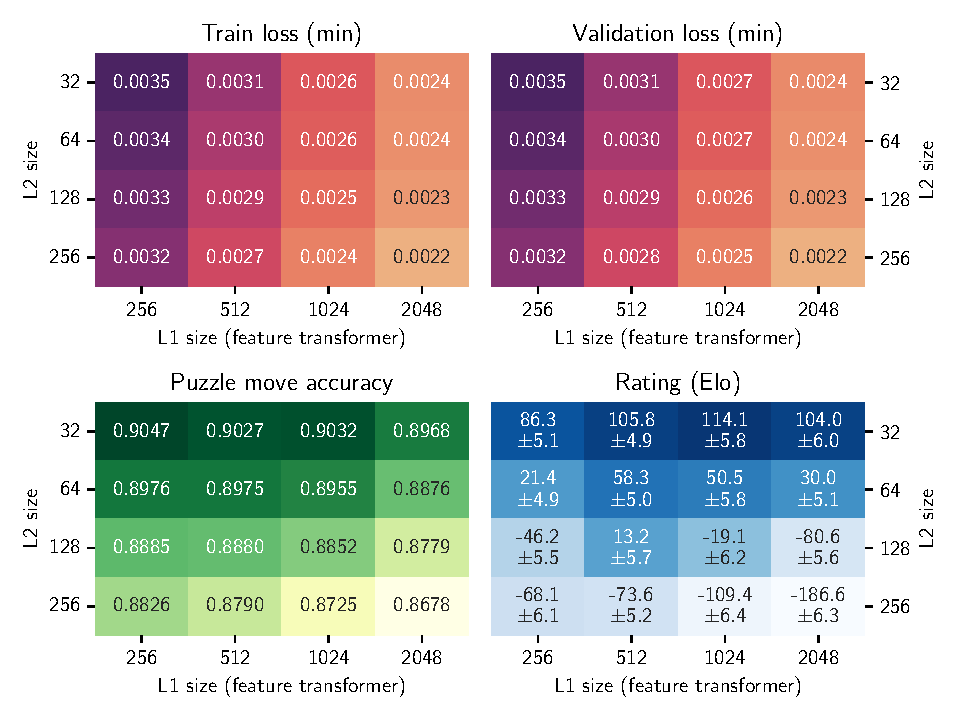
\includegraphics[width=\textwidth]{./dynamic/output/baseline_heatmaps.pdf}}
\captionsetup{justification=centering}
\caption{Network architecture sweep results (L1 $\times$ L2).\\ Table with details in Appendix \ref{appendix:baseline}.}
\label{fig:baseline_heatmaps}
\end{figure}

If L2 is kept constant, the best L1 is not the smallest nor biggest. If L2 $=64$ or L2 $=128$ there is a clear lead of L1 $=512$ in both. In the case of L2 $=32$, the best L1 is not clear because the differences in rating are small and are within margin of error, excluding L1 $=256$ which is definitely wrose. Because training lower values of L1 is faster I opted for \textbf{L1} $\bm{=512}$ due the difference being small and being the best in other L2 values.

So, further experiments will use L1 $=512$ and L2 $=32$. For reference, Stockfish currently uses L1=2560, and employ (lots of) more tricks to make it even faster. The values selected here are specific to the current implementation of the engine, since it may change if more optimizations are made (tradeoff is altered). For this reason, no further modifications to the engine were made after starting with the experiments. We can now proceed with more interesting experiments.

\subsection{Axis encodings}
\label{sec:axis_encoding}

\textbf{Motivation.} Looking back at the networks generated by \featureset{All} in baseline runs, the learned weigths of most neurons in the feature transformer layer (L1) are related with the movement pattern of the pieces. Let's take the example in Figure \ref{fig:rook_weights}, which depicts the \featureset{Square} part of the features where the role is \symrook\ Rook.

\begin{figure}[h]
\centering
\subfloat[\centering $\white$ White]{{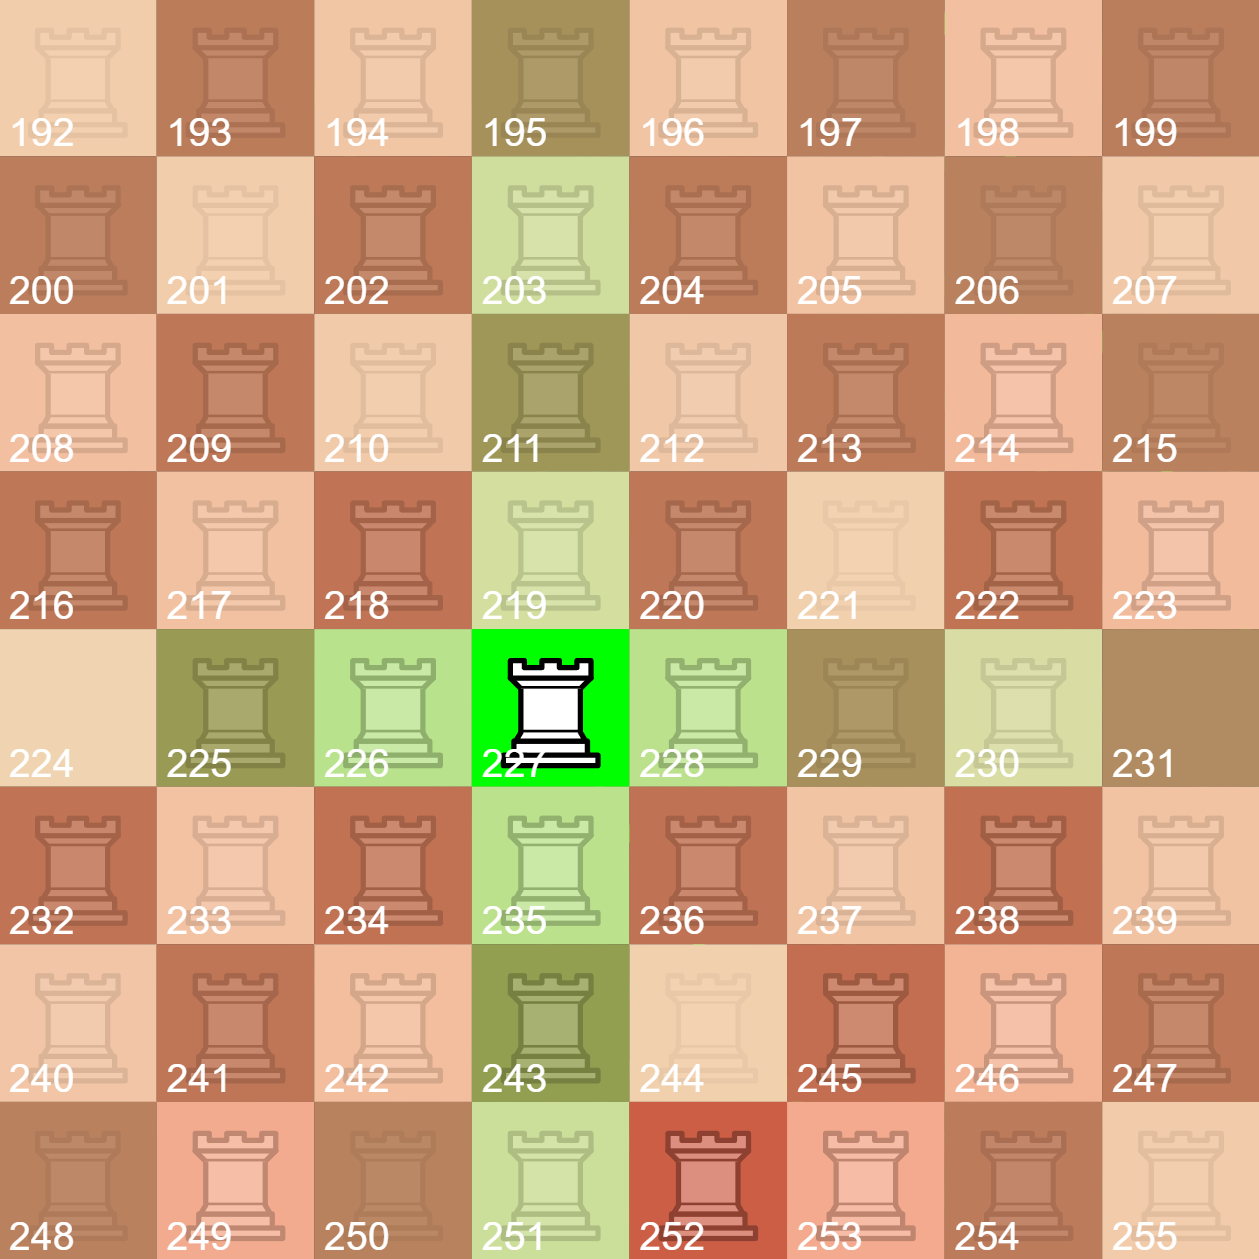
\includegraphics[width=7cm]{../assets/results/piece_weights/white_rook_weights.png} }}%
\qquad
\subfloat[\centering $\black$ Black]{{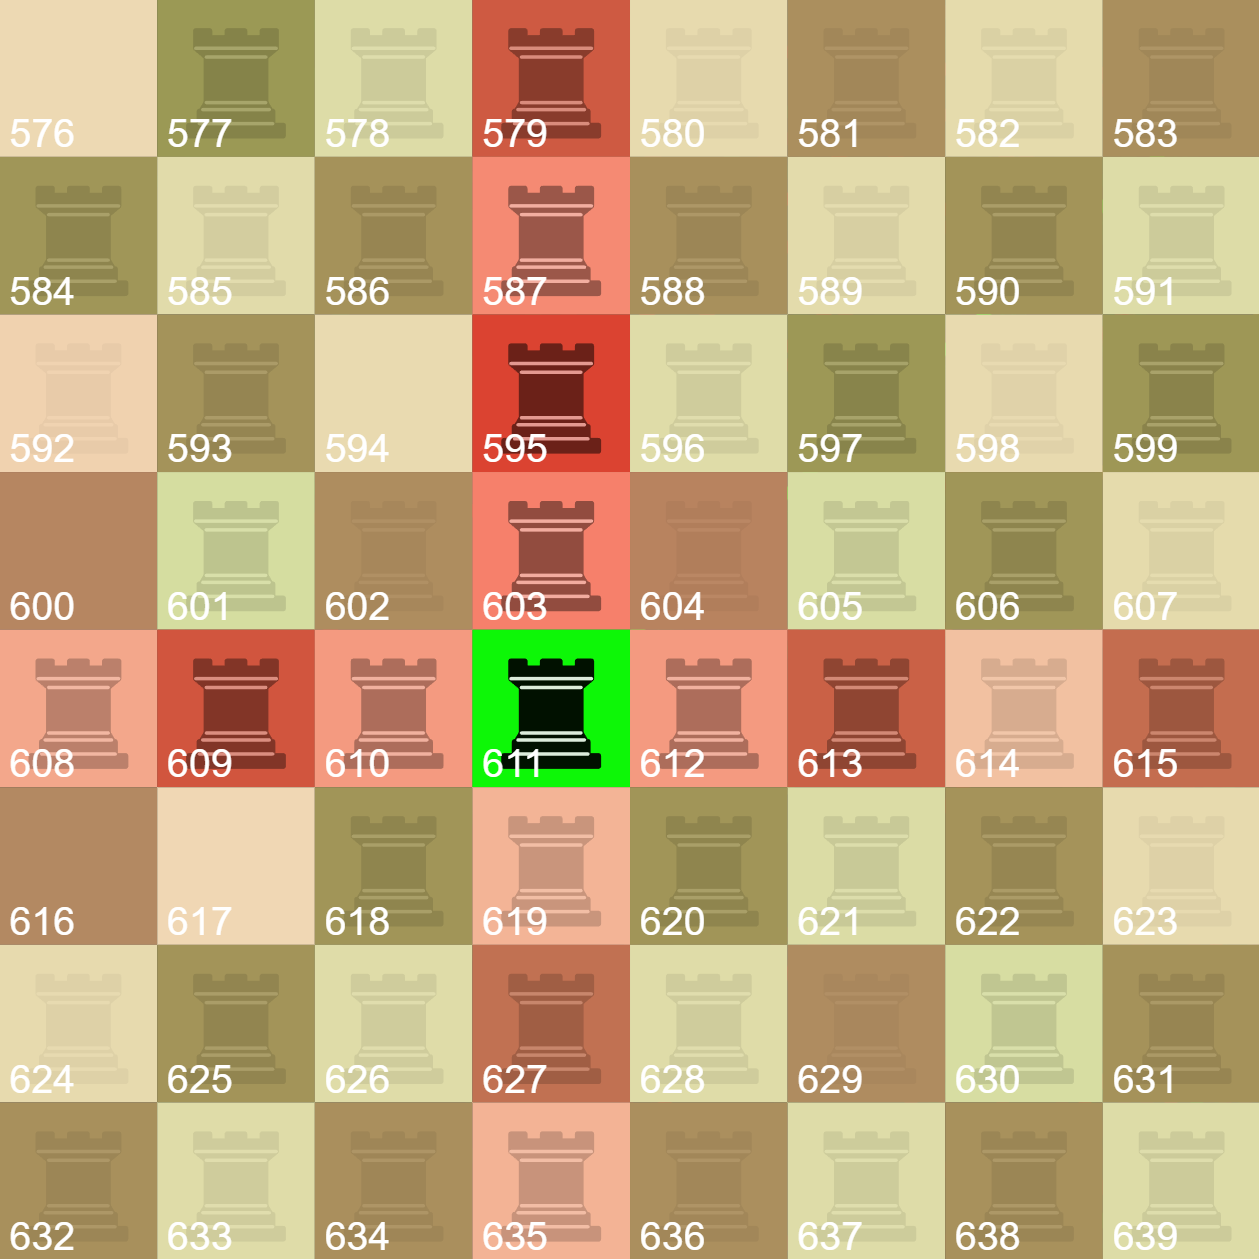
\includegraphics[width=7cm]{../assets/results/piece_weights/black_rook_weights.png} }}%
\caption{Weights of \textbf{a neuron} in the L1 layer, which are connected to features in \featureset{All} where the role is $\rook$ Rook. The intensity represents the weight value, and the color represents the sign (although not relevant).}
\label{fig:rook_weights}
\end{figure}

This particular neuron learned to recognize the presence of a \symrook\ Rook, affected by the pattern of another potential rook in the same file or rank (other pieces may be involved but I am focusing on rooks for the example). Doing so, it had to relate one feature for every potential square where a rook could be for that specific center location, which restrains the network from learning more complex patterns and it is harder to train, because you need more samples to account for all possible combinations.

What if we add a feature which describes \enquote{\textit{there is a $\white$ White $\rook$ Rook in the 4th rank}}? Certainly, this would make the network's job easier, as it would only need to learn the presence of rooks in the corresponding file or rank, instead of every square. This idea can be extrapolated to diagonals, to ease patterns with $\bishop$ Bishops and the $\queen$ Queen.

More examples of this behaviour can be found in Appendix \ref{appendix:axis_samples}, showcasing diagonal patterns and the $\knight$ Knight movements, although they do not move straight through axes. \\

\textbf{Experiment.} I built blocks of features for each natural axis of a chess board, which coincide with the movement pattern of the pieces:

\begin{table}[H]
\centering
\begin{tabular}{cccc}
\depiction{H} & \depiction{V} & \depiction{D1} & \depiction{D2} \\
Horizontal & Vertical & Diagonal 1 & Diagonal 2 \\
(across files) & (across ranks) &  & 
\end{tabular}
\end{table}

% The canonical \featureset{All} feature set encodes each piece's position using the square it is located. Note that this is the same thing as encoding the position for a piece $P$ as $\featureset{File}_{P} \times \featureset{Rank}_{P}$. So the position of each piece is determined using the vertical (across ranks) and horizonal (across files) axes.

In table \ref{tab:axes_blocks} I present the feature blocks. Each block will encode whether there is a piece with the role and color in a specific location along that axis, as explained in the example.

\begin{table}[H]
\caption{Axes feature blocks}
\label{tab:axes_blocks}
\centering

\newcommand{\fullrolecolor}{$\times$ $\featureset{Role}_{P} \times \featureset{Color}_{P}$}

\begin{tabular}{cccccc}
\toprule
\bf Depiction & \bf Block name & \multicolumn{2}{c}{\makecell{\bf Definition\\for every piece $P$ in the board}} & \bf \makecell{Number of\\features} \\
\toprule
\depiction{H} & $\featureset{H}$ & $\featureset{File}_{P}$ & \fullrolecolor & 96 \\
\depiction{V} & $\featureset{V}$ & $\featureset{Rank}_{P}$ & \fullrolecolor & 96 \\
\depiction{D1} & $\featureset{D1}$ & $\featureset{Diag1}_{P}$ & \fullrolecolor & 180 \\
\depiction{D2} & $\featureset{D2}$ & $\featureset{Diag2}_{P}$ & \fullrolecolor & 180 \\
\bottomrule
\end{tabular}

\end{table}


With this blocks, I built different feature sets (listed in table \ref{tab:axis_encoding}): one group of feature sets is just combinations of all the blocks, and another group which is the same as the first but alongside the \featureset{All} feature set (here treated as a block). The second group is the aim of the experiment, it has the classic \featureset{All} feature set but includes the axis blocks to see if the network can benefit from them. The first group, which does not include \featureset{All} is to know how far the network can go only with this blocks alone.

\begin{table}[H]
\caption{Axis encodings feature sets}
\label{tab:axis_encoding}
\centering

\newcommand{\rolecolor}{$\times$ $\featureset{R}_{P} \times \featureset{C}_{P}$}

\begin{tabular}{ccc}
\toprule
\bf Depiction & \bf Feature set & \bf \makecell{Number of\\features} \\
\toprule
\depiction{H} $\oplus$ \depiction{V} & $\featureset{H} \oplus \featureset{V}$ & 192 \\
\midrule
\depiction{D1} $\oplus$ \depiction{D2} & $\featureset{D1} \oplus \featureset{D2}$ & 360 \\
\midrule
\depiction{H} $\oplus$ \depiction{V} $\oplus$ \depiction{D1} $\oplus$ \depiction{D2} & $\featureset{H} \oplus \featureset{V}$ $\oplus$ $\featureset{D1} \oplus \featureset{D2}$ & 552 \\
\midrule
% ------------------------------------
\midrule
\featureset{All} $\oplus$ \depiction{H} $\oplus$ \depiction{V} & $\featureset{All} \oplus \featureset{H} \oplus \featureset{V}$ & 960 \\
\midrule
\featureset{All} $\oplus$ \depiction{D1} $\oplus$ \depiction{D2} & $\featureset{All} \oplus \featureset{D1} \oplus \featureset{D2}$ & 1128 \\
\midrule
\featureset{All} $\oplus$ \depiction{H} $\oplus$ \depiction{V} $\oplus$ \depiction{D1} $\oplus$ \depiction{D2} & \featureset{All} $\oplus$ \featureset{H} $\oplus$ \featureset{V} $\oplus$ \featureset{D1} $\oplus$ \featureset{D2} & 1320 \\
\bottomrule

\end{tabular}
\end{table}

I expect that the feature sets that are sums of single axes ($\depictionSM{H} \oplus \depictionSM{V}, \depictionSM{D1} \oplus \depictionSM{D2}$ and $\depictionSM{H} \oplus \depictionSM{V} \oplus \depictionSM{D1} \oplus \depictionSM{D2}$) will perform worse overall, since to capture the exact position of pieces in the board, the network will have to learn to relate at least two features for every location. This information is already available when \featureset{All} is present.

The feature sets that include \featureset{All} (\featureset{All} $\oplus \hdots$) should perform better than without, providing that the idea explained in the motivation holds.

For each of the proposed feature sets, I will train a network and evaluate its performance relative to each other using a tournament. I expect to see them ranked in the reverse order as presented in the table (more extra axes better). \\

\textbf{Results.} The results in table \ref{tab:axis_results} show that indeed, adding the axes blocks make the network validation loss slightly lower, from 0.00316 in \featureset{All} to 0.00307 including all four blocks. However, this improvement in loss is not significant enough to make the network stronger to compensate the (small) performance hit of having more features. As you can see in the table, including more axes makes the loss decrease slightly yet the rating decreases by a huge factor.

All three feature sets that do not include \featureset{All} unsuprisingly perform much, much worse even having less features. The feature set \featureset{H+V+D1+D2} has a 25\% higher loss than \featureset{All} and $172.5 \pm 4.8$ less rating than \featureset{All}. The other feature sets in this group perform even worse, as it was expected.

I discovered that the accuracy of puzzles is not a good a proxy of an engine's strength, given that there is a 474 rating difference yet 3\% a difference in move accuracy. I believe that the reason lies on the fact that puzzles may be more strategic than positional. I will drop the puzzle accuracy metric in future experiments.

\begin{table}[H]
\caption{Axis encodings results}
\label{tab:axis_results}
\centering

% 1 256-eval_16384_(hv[768]→512)x2→32→1.nn          :     0.0   ----  22665.5   32456    70      96
% 2 256-eval_16384_(hv+h+v[960]→512)x2→32→1.nn      :    -4.6    5.0  22474.0   32456    69     100
% 3 256-eval_16384_(hv+d1+d2[1128]→512)x2→32→1.nn   :   -33.3    5.0  21260.5   32456    66     100
% 4 256-eval_16384_(hv+h+v+d1+d2[1320]→512)x2→32→1.nn   :   -57.7    4.8  20207.5   32458    62     100
% 5 256-eval_16384_(h+v+d1+d2[552]→512)x2→32→1.nn   :  -172.5    4.8  15176.0   32456    47     100
% 6 256-eval_16384_(h+v[192]→512)x2→32→1.nn         :  -368.1    5.7   7527.0   32460    23     100
% 7 256-eval_16384_(d1+d2[360]→512)x2→32→1.nn       :  -474.5    6.4   4289.5   32458    13     ---

% Network: 256-eval_16384_(d1+d2[360]→512)x2→32→1.nn Accuracy: 0.851789055191768
% Network: 256-eval_16384_(h+v+d1+d2[552]→512)x2→32→1.nn Accuracy: 0.8748684518241348
% Network: 256-eval_16384_(h+v[192]→512)x2→32→1.nn Accuracy: 0.8618817235734331
% Network: 256-eval_16384_(hv+d1+d2[1128]→512)x2→32→1.nn Accuracy: 0.8814458606173995
% Network: 256-eval_16384_(hv+h+v+d1+d2[1320]→512)x2→32→1.nn Accuracy: 0.8766955098222639
% Network: 256-eval_16384_(hv[768]→512)x2→32→1.nn Accuracy: 0.8865762394761459
% Network: 256-eval_16384_(hv+h+v[960]→512)x2→32→1.nn Accuracy: 0.8851511342376053

\begin{tabular}{cccccc}
\toprule
\bf Feature set  & \bf \makecell{Number\\of features} & \makecell{\bf Val. loss\\\textit{min}} & \makecell{\bf Rating\\\textit{elo (rel. to \featureset{All})}} & \makecell{\bf Puzzles\\\textit{move acc.}} \\
\toprule
\depiction{H} $\oplus$ \depiction{V} & 192 & 0.00581 & -368.1 $\pm$ 5.7 & 0.8618 \\
\midrule
\depiction{D1} $\oplus$ \depiction{D2} & 360 & 0.00670 & -474.5 $\pm$ 6.4 & 0.8517 \\
\midrule
\makecell{\depiction{H} $\oplus$ \depiction{V} $\oplus$ \\ \depiction{D1} $\oplus$ \depiction{D2}} & 552 & 0.00389 & -172.5 $\pm$ 4.8 & 0.8748 \\
\midrule
% ------------------------------------
\midrule
\featureset{All} (reference) & 768 & 0.00316 & \textbf{0.0} & 0.8865 \\
\midrule
\featureset{All} $\oplus$ \depiction{H} $\oplus$ \depiction{V} & 960 & 0.00308 & -4.6 $\pm$ 5.0 & 0.8851 \\
\midrule
\featureset{All} $\oplus$ \depiction{D1} $\oplus$ \depiction{D2} & 1128 & 0.00309 & -33.3 $\pm$ 5.0 & 0.8814 \\
\midrule
\makecell{\featureset{All} $\oplus$ \depiction{H} $\oplus$ \depiction{V} \\ \hspace{0.75cm} $\oplus$ \depiction{D1} $\oplus$ \depiction{D2}} & 1320 & \textbf{0.00307} & -57.7 $\pm$ 4.8 & 0.8766 \\
\bottomrule

\end{tabular}
\end{table}

The next experiment will focus on adding more specific features, instead of more broad ones.


\subsection{Pairwise axes}

\textbf{Motivation.} Imagine that in a file there are three pieces: an enemy $\symrook$ Rook, a $\sympawn$ Pawn and a $\symknight$ Knight. There are many possible configurations for these pieces on the file. The influence in the evaluation by those pieces is very related with the position of pieces everywhere else, however I want to see if to understand a single file, the actual position of the pieces is less important than the relative order between them: $\sympawn\symknight\symrook, \sympawn\symrook\symknight, \symknight\sympawn\symrook, \symknight\symrook\sympawn, \symrook\sympawn\symknight, \symrook\symknight\sympawn$. In other words, provide the network features based on the order of the pieces instead of the actual position. This way, I believe that the network can pick up whether pieces are pinned, protected by other pieces or can attack other pieces.

I propose to make a feature for each possible pair of adjacent role and color over an axis. Lets consider the \textit{a} file (vertical axis), following the example before:

\storechessboardstyle{smallvert}{
    tinyboard,
    maxfield=a8,
    showmover=false,
    hmargin=false,
    hlabel=false,
    boardfontsize=15pt,
}

\newcommand{\raiseby}{-11.5ex}

\begin{figure}[H]
\centering

\begin{tabular}{ccc}

\raisebox{\raiseby}{\chessboard[
    style=smallvert,
    addblack={Ra7},
    addwhite={na3,pa4},
]}
\raisebox{\raiseby}{\chessboard[
    style=smallvert,
    addblack={Ra8},
    addwhite={na2,pa3},
]}
\raisebox{\raiseby}{\chessboard[
    style=smallvert,
    addblack={Ra6},
    addwhite={na3,pa4},
]}
\raisebox{\raiseby}{\chessboard[
    style=smallvert,
    addblack={Ra5},
    addwhite={na1,pa3},
]}
\raisebox{\raiseby}{\chessboard[
    style=smallvert,
    addblack={Ra6},
    addwhite={na2,pa3},
]}

$\hdots$

&
$ \rightarrow$
&

\raisebox{-9.5ex}{\chessboard[
    blackfieldcolor=white,
    blackfieldmaskcolor=white,
    maxfield=a8,
    style=smallvert,
    vlabel=false,
    border=false,
    trim=false,
    opacity=0.6,
    addblack={Ra6},
    addwhite={na2,pa4},
    %
    color=red,
    shortenend=1.88ex,shortenstart=1.88ex, % espacio
    padding=-1ex,
    markstyle=leftborder,
    linewidth=0.4ex,
    markregion=a4-a6,
    linewidth=1.6ex,
    pgfstyle=circle,
    markfields={a4,a6},
    %
    color=blue,
    shortenend=1.88ex,shortenstart=1.88ex, % espacio
    padding=-1ex,
    markstyle=leftborder,
    linewidth=0.4ex,
    markregion=a2-a4,
    linewidth=1.6ex,
    pgfstyle=circle,
    markfields={a2,a4},
    %
]}

\\

\makecell{Different configurations,\\similar situation} &  & \makecell{The same two features\\(blue pair and red pair)}

\end{tabular}
\end{figure}

There are many configurations for the three pieces and the idea is to collapse all of these into two features: the pair of pieces ($\symrook$$\black$, $\sympawn$$\white$) and the pair of pieces ($\sympawn$$\white$, $\symknight$$\white$). This way, the network can learn that the $\symrook$ Rook can capture the $\sympawn$ Pawn, and that the $\symknight$ Knight is protected behind the $\sympawn$ Pawn. The network can learn this situation using two features instead of learning it for every possible configuration.

In contrast to the previous experiment where the features were more general (\textit{\enquote{there is a $\white$ White $\rook$ Rook in the 4th rank}}) the proposed features here are more specific: \textit{\enquote{there is a $\black$ Black $\rook$ Rook next to a $\white$ White $\sympawn$ Pawn in the \enquote{a} file}}. \\

\textbf{Experiment.} I developed two feature blocks: for the horizonal and vertical axis. The blocks are defined in table \ref{tab:pairwise_blocks}:

\begin{table}[H]
\caption{Pairwise feature blocks}
\label{tab:pairwise_blocks}
\centering

\begin{tabular}{ccccc}
\toprule
\bf Depiction & \bf \makecell{Block\\name} & \bf Definition & \bf \makecell{Num. of\\features} \\
\toprule
\depiction{PH} & PH & \makecell{
\vspace{0.2cm}
$(\featureset{Ranks} \times (\featureset{Roles} \times \featureset{Colors}) \times (\featureset{Roles} \times \featureset{Colors}))_{P}$ \\
P($\langle r, r_1, c_1, r_2, c_2 \rangle$): there is a piece in rank $r$ with role $r_1$\\ and color $c_1$ to the left of a piece with role $r_2$ and color $c_2$
} & 1152 \\
\toprule
\depiction{PV} & PV & \makecell{
\vspace{0.2cm}
$(\featureset{Files} \times (\featureset{Roles} \times \featureset{Colors}) \times (\featureset{Roles} \times \featureset{Colors}))_Q$ \\
Q($\langle f, r_1, c_1, r_2, c_2 \rangle$): there is a piece in file $f$ with role $r_1$\\ and color $c_1$ below a piece with role $r_2$ and color $c_2$
} & 1152 \\
\bottomrule
\end{tabular}
\end{table}

Note that it is important to consider the order of the pieces in the pair, as expressed in the direction of the definition (left and below).
This makes sure features are not mirrored, since we want to differentiate between both. In code this is handled by iterating over the pieces and building the pair in the same order every time.

The following figure shows what pairs of pieces (features) are considered for the horizonal and vertical axes in a complete board:

\begin{figure}[H]
\centering
\begin{tabular}{cc}

\raisebox{-7ex}{\chessboard[
    setfen=2r4k/p5p1/Kpqp3p/8/1PP2Q2/P2P1RP1/8/8 b - - 12 45,
    showmover=false,
    opacity=0.6,
    %
    % TEMPLATE HORIZONTAL
    %color=red,
    %shortenend=1.88ex,shortenstart=1.88ex, % espacio
    %padding=-1ex,
    %markstyle=topborder,
    %linewidth=0.4ex,
    %markregion=d6-d3,
    %linewidth=1.6ex,
    %pgfstyle=circle,
    %markfields={d6,d3},
    %
    color=red,
    shortenend=1.88ex,shortenstart=1.88ex, % espacio
    padding=-1ex,
    markstyle=topborder,
    linewidth=0.4ex,
    markregion=a3-d3,
    linewidth=1.6ex,
    pgfstyle=circle,
    markfields={a3,d3},
    %
    color=red,
    shortenend=1.88ex,shortenstart=1.88ex, % espacio
    padding=-1ex,
    markstyle=topborder,
    linewidth=0.4ex,
    markregion=f3-g3,
    linewidth=1.6ex,
    pgfstyle=circle,
    markfields={f3,g3},
    %
    color=blue,
    shortenend=1.88ex,shortenstart=1.88ex, % espacio
    padding=-1ex,
    markstyle=topborder,
    linewidth=0.4ex,
    markregion=d3-f3,
    linewidth=1.6ex,
    pgfstyle=circle,
    markfields={d3,f3},
    %
    color=red,
    shortenend=1.88ex,shortenstart=1.88ex, % espacio
    padding=-1ex,
    markstyle=topborder,
    linewidth=0.4ex,
    markregion=b4-c4,
    linewidth=1.6ex,
    pgfstyle=circle,
    markfields={b4,c4},
    %
    color=blue,
    shortenend=1.88ex,shortenstart=1.88ex, % espacio
    padding=-1ex,
    markstyle=topborder,
    linewidth=0.4ex,
    markregion=c4-f4,
    linewidth=1.6ex,
    pgfstyle=circle,
    markfields={c4,f4},
    %
    color=red,
    shortenend=1.88ex,shortenstart=1.88ex, % espacio
    padding=-1ex,
    markstyle=topborder,
    linewidth=0.4ex,
    markregion=a6-b6,
    linewidth=1.6ex,
    pgfstyle=circle,
    markfields={a6,b6},
    %
    color=red,
    shortenend=1.88ex,shortenstart=1.88ex, % espacio
    padding=-1ex,
    markstyle=topborder,
    linewidth=0.4ex,
    markregion=c6-d6,
    linewidth=1.6ex,
    pgfstyle=circle,
    markfields={c6,d6},
    %
    color=blue,
    shortenend=1.88ex,shortenstart=1.88ex, % espacio
    padding=-1ex,
    markstyle=topborder,
    linewidth=0.4ex,
    markregion=b6-c6,
    linewidth=1.6ex,
    pgfstyle=circle,
    markfields={b6,c6},
    %
    color=blue,
    shortenend=1.88ex,shortenstart=1.88ex, % espacio
    padding=-1ex,
    markstyle=topborder,
    linewidth=0.4ex,
    markregion=d6-h6,
    linewidth=1.6ex,
    pgfstyle=circle,
    markfields={d6,h6},
    %
    color=red,
    shortenend=1.88ex,shortenstart=1.88ex, % espacio
    padding=-1ex,
    markstyle=topborder,
    linewidth=0.4ex,
    markregion=a7-g7,
    linewidth=1.6ex,
    pgfstyle=circle,
    markfields={a7,g7},
    %
    color=blue,
    shortenend=1.88ex,shortenstart=1.88ex, % espacio
    padding=-1ex,
    markstyle=topborder,
    linewidth=0.4ex,
    markregion=c8-h8,
    linewidth=1.6ex,
    pgfstyle=circle,
    markfields={c8,h8},
]}

&

\raisebox{-7ex}{\chessboard[
    setfen=2r4k/p5p1/Kpqp3p/8/1PP2Q2/P2P1RP1/8/8 b - - 12 45,
    showmover=false,
    opacity=0.6,
    %
    % TEMPLATE VERTICAL
    %color=red,
    %shortenend=1.88ex,shortenstart=1.88ex, % espacio
    %padding=-1ex,
    %markstyle=leftborder,
    %linewidth=0.4ex,
    %markregion=d6-d3,
    %linewidth=1.6ex,
    %pgfstyle=circle,
    %markfields={d6,d3},
    %
    color=red,
    shortenend=1.88ex,shortenstart=1.88ex, % espacio
    padding=-1ex,
    markstyle=leftborder,
    linewidth=0.4ex,
    markregion=a3-a6,
    linewidth=1.6ex,
    pgfstyle=circle,
    markfields={a3,a6},
    %
    color=blue,
    shortenend=1.88ex,shortenstart=1.88ex, % espacio
    padding=-1ex,
    markstyle=leftborder,
    linewidth=0.4ex,
    markregion=a6-a7,
    linewidth=1.6ex,
    pgfstyle=circle,
    markfields={a6,a7},
    %
    color=red,
    shortenend=1.88ex,shortenstart=1.88ex, % espacio
    padding=-1ex,
    markstyle=leftborder,
    linewidth=0.4ex,
    markregion=b4-b6,
    linewidth=1.6ex,
    pgfstyle=circle,
    markfields={b4,b6},
    %
    color=red,
    shortenend=1.88ex,shortenstart=1.88ex, % espacio
    padding=-1ex,
    markstyle=leftborder,
    linewidth=0.4ex,
    markregion=c4-c6,
    linewidth=1.6ex,
    pgfstyle=circle,
    markfields={c4,c6},
    %
    color=blue,
    shortenend=1.88ex,shortenstart=1.88ex, % espacio
    padding=-1ex,
    markstyle=leftborder,
    linewidth=0.4ex,
    markregion=c6-c8,
    linewidth=1.6ex,
    pgfstyle=circle,
    markfields={c6,c8},
    %
    color=red,
    shortenend=1.88ex,shortenstart=1.88ex, % espacio
    padding=-1ex,
    markstyle=leftborder,
    linewidth=0.4ex,
    markregion=d3-d6,
    linewidth=1.6ex,
    pgfstyle=circle,
    markfields={d3,d6},
    %
    color=red,
    shortenend=1.88ex,shortenstart=1.88ex, % espacio
    padding=-1ex,
    markstyle=leftborder,
    linewidth=0.4ex,
    markregion=f3-f4,
    linewidth=1.6ex,
    pgfstyle=circle,
    markfields={f3,f4},
    %
    color=red,
    shortenend=1.88ex,shortenstart=1.88ex, % espacio
    padding=-1ex,
    markstyle=leftborder,
    linewidth=0.4ex,
    markregion=g3-g7,
    linewidth=1.6ex,
    pgfstyle=circle,
    markfields={g3,g7},
    %
    color=red,
    shortenend=1.88ex,shortenstart=1.88ex, % espacio
    padding=-1ex,
    markstyle=leftborder,
    linewidth=0.4ex,
    markregion=h6-h8,
    linewidth=1.6ex,
    pgfstyle=circle,
    markfields={h6,h8},
]}


\\

\makecell{\depiction{PH} Pairwise horizontal (\featureset{PH})} &
\makecell{\depiction{PV} Pairwise vertical (\featureset{PV})}

\end{tabular}
\end{figure}

Since the blocks need at least two pieces to generate a feature, if there is only one piece over an axis, there are no active features. So, this blocks can't be used alone, they need to be combined with other features that provide that information. The most obvious choice is to combine them with the \featureset{All} block.

The feature sets to be evaluated are \featureset{All} $\oplus$ \featureset{PH} (1920 features), \featureset{All} $\oplus$ \featureset{PV} (1920 features) and \featureset{All} $\oplus$ \featureset{PH} $\oplus$ \featureset{PV} (3072 features). Like before, a network will be trained for each feature set and a tournament will be played to determinate the relative elo to the \featureset{All} baseline.

I expect that the networks are able to take advantage of the specific features, enough to conteract the loss in performance due to the big increase in the number of features and slower updates. \\

\textbf{Results.} The results in table \ref{tab:pairwise_results} show that there is a clear difference in performance between \depictionSM{PH} and \depictionSM{PV}. The feature set \featureset{All} $\oplus$ \depictionSM{PV} has a lower loss and rating than its counterpart \featureset{All} $\oplus$ \depictionSM{PH}. It is not clear why the vertical pairs achieve a better rating than the horizontal pairs, since they have a similar amount of feature updates (Appendix \ref{appendix:fs}).

Both \featureset{All} $\oplus$ \depictionSM{PV} and \featureset{All} $\oplus$ \depictionSM{PH} perform worse than \featureset{All}. It seems that the networks were able to take advantage of the pairs, since the loss is lower than the reference. However, it is not enough to conteract the increase in feature updates.

Suprisingly the feature set with both axes (\featureset{All} $\oplus$ \depictionSM{PH} $\oplus$ \depictionSM{PV}) has a similar rating to \featureset{All} $\oplus$ \depictionSM{PV}, probably counteracted by having an even lower loss.

\begin{table}[H]
\caption{Pairwise encodings results}
\label{tab:pairwise_results}
\centering

\begin{tabular}{ccccc}
\toprule
\bf Feature set  & \bf \makecell{Number\\of features} & \makecell{\bf Val. loss\\\textit{min}} & \makecell{\bf Rating\\\textit{elo (rel. to \featureset{All})}} \\
\toprule
\featureset{All} (reference) & 768 & 0.003134 & \textbf{0.0} \\
\midrule
\featureset{All} $\oplus$ \depiction{PH} & 1920 & 0.003033 & -38.2 $\pm$ 4.8 \\
\midrule
\featureset{All} $\oplus$ \depiction{PV} & 1920 & 0.002946 & -8.4 $\pm$ 5.0 \\
\midrule
\featureset{All} $\oplus$ \depiction{PH} $\oplus$ \depiction{PV} & 3072 & \textbf{0.002868} & -37.6 $\pm$ 4.9 \\
\bottomrule
\end{tabular}
\end{table}

Future work could gather some statistics about the pairs and determinate if skipping some pairs is worth it. For example, pairs related to pawns cause many updates since it is the most common piece and may not be that useful. Reducing the amount of pairs would lower the amount of updates and may overtake \featureset{All}.

I did not bother implementing diagonal pairs (\depiction{PD1} and \depiction{PD2}) due the adverse result of the other axes.


